\chapter{Awareness, comments, evaluation}
\label{prod.res.qual}

Up to now, the focus of this study has been exclusively on \emph{how} subjects say things.
In what is to follow I will present a short summary of \emph{what} the people in my sample have to say \emph{about} Scouse, zooming in on the opinions expressed and the comments made in the interview sections on (local) \isi{identity} and language.
This analysis can only be qualitative in nature due to the fact that the number of interviewees is far too small to permit meaningful quantitative comparisons.
It should also be considered recapitulatory, as constraints of time and space do not allow me to provide a comprehensive analysis of all the material that was collected at this point.
\figref{fig.aware.nurse} and \figref{fig.aware.k} are based on data extracted from all 38 interviews that have been conducted (the `secondary sample'), but the more detailed description on the following pages focuses on the same 20 participants that provided the data for the quantitative analyses reported in Chapters \ref{ch.prod_results_vow} and \ref{prod.res.con} (the `primary sample', cf. \sectref{sec.prod_method.participants}).
Quotes are attributed to the relevant interviews using the participant codes explained in \sectref{sec.prod_method.interview}.
For reasons of readability, hesitations and repetitions in these quotes have been eliminated.

\section{Scouse and `Liverpoolness'}

\subsection{Accent and identity}

It is not really surprising that the question of \isi{identity} is intertwined with the question of language (variety) for many people.
Nevertheless, it is interesting how strongly these two concepts are linked up by many subjects in my sample.
The most explicit comment on this issue probably stems from a male, middle-class speaker who states: ``We got our \isi{identity}, haven't we. We talk different'' (01MMC52).
A female who is some 30 years younger made a statement whose gist is very similar:
\begin{example}
	I'd call meself a Scouser\is{identity} 'cause I always called meself that. I don't know why. (\ldots) We've got a Scouse accent, we're labelled as Scouser\is{identity}s. (37FWC20)
\end{example}
Having a Scouse accent thus seems to be, for her, essentially the same thing as \emph{being} a Scouser\is{identity}.
While many subjects consider the terms `Liverpudlian\is{identity}' and `Scouser\is{identity}' to be synonyms, broadly speaking, there are still quite a few for who these terms carry somewhat different connotations.
The speaker quoted at the beginning of this paragraph, for instance, says that, although he ``wouldn't be offended if someone said [he] was a Scouser\is{identity}'', he nevertheless prefers the term `Liverpudlian\is{identity}' to refer to himself, because he ``just sound[s] a Liverpudlian\is{identity}'' (01MMC52).

While this subject does not go on to explain what distinguishes a Liverpudlian\is{identity} from a Scouser\is{identity} in terms of `sound', a young female speaker in the sample is more explicit on the issue.
\begin{example}
	I'd never call myself [a Scouser\is{identity}] 'cause I don't sound very Scouse compared to others. So I think it's to do with the sort of, how strong your accent is. (06FMC20)
\end{example}
Another female of the same age group voices essentially the same idea by explaining that ``people tend to think of Scouser\is{identity}s, you know with the really strong accent'' (07FMC23), and that, since she didn't have a strong accent, she was reluctant to refer to herself as a Scouser\is{identity}.
It should be noted, however, that the issue is more complicated than that for at least some people from Liverpool.
A not insignificant proportion of interviewees explained that the term `Liverpudlian\is{identity}' was ambiguous for them, because it could either mean
\begin{inparaenum}[(1)]
	\item `someone from Liverpool', or
	\item `someone supporting Liverpool Football Club'.
\end{inparaenum}
Since the football allegiance is quite important for many people in Liverpool, `Evertonians' (supporters of Everton, the other premier league football club in the city) often rejected the label `Liverpudlian\is{identity}' and would go for `Scouser\is{identity}' instead, simply because they wanted to avoid being `misunderstood'.

\subsection{Distinctness, geographical spread, and `plastic' Scousers}

Notwithstanding these minor terminological issues, subjects in different age groups express the thought that a Liverpool accent might be particularly closely linked to a Liverpool \isi{identity} because it is so distinct\is{distinctness}ive.
A 20-year old working-class male, for instance, claims that Scouser\is{identity}s were ``instantly recognisable'' because of the ``distinct\is{distinctness}ive accent'' (02MWC20), and a 44-year-old female (talking about people from Manchester in particular) says that ``the minute they hear you talk (\ldots) you see a little light go on in there'' (13FWC44).
Another subject from the middle-aged group hypothesises about whether Liverpool as a city might be stigmatise\is{stigmatisation}d because ``you can pick a Scouser\is{identity} a mile off'' thanks to the distinct\is{distinctness}ive accent.
He even goes on to compare Scouse as a city accent to that of \isi{Lancashire} as a regional one, arguing that Manchester, as a city, does not have its own accent in the same way that Liverpool does:

\begin{example}
	Someone from Manchester may sound as if they were from any number of towns (\ldots) They're gonna be lumped together, (\ldots) but there's a relatively small number of people who are Liverpudlian\is{identity} or sound Liverpudlian\is{identity} and so (\ldots) maybe it's the distinct\is{distinctness}iveness which is what makes it an easy target. (03MMC33)
\end{example}

The same speaker also claims, that -- in his opinion -- the accents of places such as London or Newcastle ``sound (\ldots) a lot more similar than Liverpudlian\is{identity} does to anything else'' (03MMC33).
This seems like a rather drastic interpretation of the distinct\is{distinctness}ness of Scouse, and I cannot say whether this idea is embraced by a majority of Liverpudlians, but one of the younger subjects even went one step further and admitted to feeling ``a sense of detachment sometimes'', supposedly ``'cause the accent's so different\is{distinctness} from the rest of England'' (02MWC20).

While many speakers in my sample are quite happy about, and take some pride in, the fact that their accent is (considered as) rather distinct\is{distinctness}, both the 33-year-old middle-class speaker and the 20-year-old working-class interviewee just quoted also see this distinct\is{distinctness}ness as somewhat ambivalent.
The older one refers to potentially negative effects indirectly when he says that the distinct\is{distinctness}ness of the accent makes Liverpool ``an easy target''.
The younger speaker, on the other hand, explicitly laments that ``sometimes'' outsiders linked the accent to ``the negative \isi{stereotype}[s]'' about Liverpool\is{image}, a fact which he considers as somewhat unfair because the city has ``kind of evolved over the last (\ldots), like, 20 years'' and was ``certainly a modern place now\is{image}'' (02MWC20).

Notwithstanding that most speakers in the sample consider Scouse to be so characteristic of the city, Liverpudlians of all age groups are also aware\is{awareness} of the fact that speakers of Scouse can be found outside of the city limits.
However, these people are often thought of as `fake', or `plastic\is{plastic Scouse(r)}' Scouser\is{identity}s in the local terminology (cf. \emph{crossing} as defined by \citealt{rampton1995}).
Definitions vary as to where exactly plastic\is{plastic Scouse(r)} Scouser\is{identity}s are to be found.
For some people they ``live in Birkenhead and Wallasey'' (06FMC20), i.e. on the \isi{Wirral} peninsula to the west of Liverpool.
A person from there might have a way of speaking that is ``classed [as] a Scouse accent'', but they are still ``not a real Scouser\is{identity}'' because they live ``over the water'' (06FMC20).
For many Liverpudlians this is true even though many of the plastic\is{plastic Scouse(r)} Scouser\is{identity}s actually have rather strong Liverpudlian accents as one speaker explained, who first talked about a (Liverpudlian\is{identity}) acquaintance with ``a really thick accent'' and then went on to explain that ``you find people of the other side of the river talk like him'' (01MMC52).
Also frequently labelled as plastic\is{plastic Scouse(r)} Scouser\is{identity}s are people who live to the north or east of Liverpool `proper': they are not separated from the city by the natural border of the Mersey estuary, but they nevertheless live outside the administrative boundaries of the city itself.
Sometimes this even refers to people who live within the contiguously built-up area of the Liverpool city region (such as in Halewood or Huyton).
For most subjects, however, plastic\is{plastic Scouse(r)} Scouser\is{identity}s are to be found a bit further away from the centre.
For instance, a 38-year-old woman in my sample included people from ``St. Helens or Skelmersdale or (\ldots) Warrington'' (around 22km, 41km, and 28km from Liverpool, respectively) in this category and gave ``Mel C of the Spice Girls'' and the comedian John Bishop as celebrity examples (33FMC38).
Incidentally, she also thinks that the latter's accent is ``the worst'', which serves to illustrate another aspect often connected with the term plastic\is{plastic Scouse(r)} Scouser\is{identity}, namely the idea that ``they put it on too much'', i.e. that they perform\is{accent performance} an inauthentic\is{authenticity} and exaggerated Scouse accent (33FMC38).

\subsection{In the north, but not of it?}
\label{aware_res.north}

There is thus wide-spread aware\is{awareness}ness both of the distinct\is{distinctness}ness of Scouse and its close connection with the city of Liverpool.
All the same, neither the ideas about the distinct\is{distinctness}ness of Scouse, nor the views expressed about so-called plastic\is{plastic Scouse(r)} Scouser\is{identity}s should be taken to mean that Liverpudlians across the board necessarily think that their city is absolutely unique and not part of any larger cultural region.
To assess subjects' \isi{attitude}s and opinions in this respect they were asked whether they would describe themselves as northerner\is{identity}s and they were confronted with the phrase Liverpool is ``in the north but not of it'' \parencite[xxx]{belchem2006b}.
Reactions were quite diverse.

Older speakers in my sample seem to be most willing to embrace the idea that Liverpool is separate and not really part of northern England in the same way that other cities such as Manchester, Leeds, or Sheffield are.
One of the older males, for instance, does concede that he ``[is] northern'', but then adds that it was really ``too broad a term for someone from Liverpool'' and that it might better ``suit someone from \isi{Lancashire} or Yorkshire'', whereas people from Liverpool were (primarily) Scouser\is{identity}s (08MMC62).
To be fair, this person also points out that, in his opinion, the claim that Liverpool is separate from the rest of the north was ``less true'' today, but that ``it certainly was very true at one point, 'cause Liverpool just had a different \isi{attitude} to the rest of the country''.
Now, however, he would not strongly object to Liverpool being called a ``northern'' city anymore (08MMC62).
Another male speaker of about the same age is more categorical and insists that Liverpool is ``distinct\is{distinctness}'', ``not like, say, Manchester'', and ``nothing like Birmingham'', even though the former is ``just a hop, skip, and a jump down the road'' (05MWC66).
Interestingly, he even provides some historical justification for his opinion, arguing that Liverpool is characterised by
\begin{inparaenum}[(1)]
	\item a ``mix of \isi{Welsh}, \isi{Irish}, some \isi{Scottish}, and (\ldots) \isi{Lancashire}'',
	\item its peripheral geographical position in the country (``it's physically just that big way out''), and
	\item ``that seafaring thing'', i.e. the tradition as an important port which meant that the orientation of Liverpool was ``always outwards'' (05MWC66).
\end{inparaenum}

The two women in the old group seem to have somewhat more `moderate' views in this respect, but since the sample is so small it is unclear whether this is a true gender difference that could be generalised to the majority of Liverpudlians.
The working-class subject, for instance, claims that she has ``always been northern'' in addition to her Liverpool \isi{identity}.
She does not deny that the ``Liverpudlian\is{identity} bit [comes] first'', and that the northern \isi{identity} is secondary, but she does think that Liverpool is ``part of northern England'' (18FWC67).
The other older female in the sample, like many others, does attribute a ``bit of a stand alone quality maybe to Liverpool'', but she is also very aware\is{awareness} of ``that \isi{north-south divide}'' and explains that, on a recent trip to Oxfordshire, she had ``really felt very northern'' (28FMC59).
While she also feels ``there is a difference'' between Liverpool and other places in the north of England, this does not keep her from including Liverpool in the north.
Interestingly, she also suggests that the idea of uniqueness is an important aspect of Liverpool's \isi{identity}:
\begin{example}
	No, I don't think Liverpool's separate. I think Liverpool likes to \emph{think} it's separate to the (\ldots) rest of the north (\ldots). I don't feel it is. (28FMC59, emphasis in the original)
\end{example}

In the middle age group, one also finds people who believe that Liverpool is ``more unique'' than other places in northern England, but they usually put this into perspective by saying something like ``but I wouldn't necessarily say it was separate'' (33FMC38): Liverpool is thus considered somewhat special, but special \emph{within} the group of northern English cities and towns.
Other speakers even consider Liverpool to be a prototypical northern city which ``absolutely shows what (\ldots) a northerner\is{identity} should be'' (13FWC44).
A male interviewee states he knows people who consider their city to be separate from everything else, but he adds it would be ``such a shame if Liverpool wasn't able to relate to the rest of \isi{Lancashire}'' and ``other places in northern England'', and explains that he himself is ``happy being of the north'' (03MMC33).

The youngest speakers are again slightly more homogeneous when it comes to the issue of northernness.
One of them limits Liverpool's association with the north to a purely geographical one (``we are in the north'') and does not see any cultural similarities between Liverpudlian\is{identity}s and northerner\is{identity}s who ``dress different'' and ``walk different'' (37FWC20).
Liverpool is considered to be ``different from northern cities'' and ``sort of unique'', with its own ``different way of life, really'' (37FWC20).
A male working-class speaker of the same age group reverses the argument presented by one of the older speakers, and explains that ``in the 80s and such [Liverpool] was definitely a part of the north, like a solid part of the north'', whereas nowadays the city was ``so detached from northern places'' that he had ``never thought of [himself] as [a] northerner\is{identity}'' (02MWC20).
The accent issue is brought up again by one of the young women, who believes that typical ``northern people'' are thought of as having ``quite broad northern accent[s]'', which are more likely to be found in places ``like Leeds or Yorkshire, or somewhere like that maybe'' (07FMC23).
The intermediate position is also found, where Liverpool is special, but not too different from other places to be included in the `northern' category, especially against the backdrop of the \isi{north-south divide}:
\begin{example}
	Our culture isn't the same as a lot of the other northern cities, but it's not exactly the same as the south.
	It's a very unique city, I suppose (...).
	I think it is northern, but in a rather distinct\is{distinctness} way. (04MWC19)
\end{example}

Generally speaking, though, most younger Liverpudlians in my sample are quite happy with a secondary \isi{identity} as a northerner\is{identity} -- especially those that have travelled more, or have family in other parts of the country (north and south).
One working-class female, for example, does not even see a ``drastic difference between Liverpool and Manchester'', the two historical `arch-enemies' in the north-west, whereas the difference ``between the north and south'' is much more important to her (36FWC20).
She explains that she has been to ``other places'' in northern England that just ``remind[ed] [her] of Liverpool'' instead of making her feel like she was ``miles and miles away from home because the culture's so different'' (36FWC20).
Other subjects in this age group express similar thoughts, explicitly rejecting the idea of Liverpool's separateness as ``false'' and ``just silly'', and adding that they would most certainly ``call [themselves] a northerner\is{identity}'' (06FMC20).
Context does play a crucial role here.
A male middle-class Liverpudlian can serve as a typical example when he specifies that ``in Liverpool'' he would naturally call himself ``a Scouser\is{identity}'', but if he was ``talking to (\ldots) someone from the south of (\ldots) England, [he]'d call [himself] a northerner\is{identity}'' (25MMC19).
`Northerner\is{identity}' is thus clearly a \emph{secondary} \isi{identity}, but nonetheless one that is still acceptable to (and often even readily embraced by) the youngest Liverpool speakers in the sample as a means of distancing themselves from the southern part of the country and associating with the northern one at the same time.

\section{Features of Scouse}

\subsection{Geographical variation}

Upon being asked for typical features of the Scouse accent, many subjects in my sample start out by stressing a point which an older working-class male makes very concisely when he says:
\begin{example}
	There's no such thing as a single Scouse accent. There're several Scouse accents. (05MWC66)
\end{example}
Most interviewees simply refer to the fact that `stronger' and `lighter' accents can be heard in the city, without necessarily being aware\is{awareness} of any system that might be distinguishable with respect to who uses one or the other.
The speaker who provided the last quote, however, goes on to specify that Scouse ``varies from age to age, and area to area'' and that ``some people say there's a (\ldots) very general division north and south'', with the accent arguably being ``softer in the south of the city rather than the north'' (05MWC66).
Another male speaker from the same age group also thinks that he is often able to distinguish whether someone comes ``from North Liverpool or South Liverpool'' (08MMC62).
He adds that this was particularly true ``if they're older, because South Liverpool had a much softer accent'' (08MMC62).
This conditional and the past tense that follows it suggest that he believes this distinction is less important or pronounced these days.
It still plays a role in some people's minds, however, as a quote from an older female shows.
She explains that ``if you listen to (\ldots) the boys and girls from the north end of the city, there's a real difference how they (\ldots) speak compared to here'' (28FMC59), where `here' refers to Aigburth, a middle-class suburb in the south of Liverpool.
Some speakers seem to hold very similar beliefs without actually verbalising them in such a direct manner.
As an example, consider the following quote:
\begin{example}
	The guy behind the bar, he's got a really strong accent. I think he's from Anfield. (01MMC52)
\end{example}
This speaker does not explicitly talk about different accents in different parts of Liverpool during his interview, but he nevertheless clearly makes a connection between a strong accent and a particular (northern) district of the city, Anfield, which is evidence that he does, in fact, believe that certain districts of Liverpool can be linked to stronger accents (at least in some cases).

As an aside, it should be mentioned that my subjects are probably right when they assume stronger accents to be more prevalent in northern parts of (inner-city) Liverpool.
Contrary to what many of my subjects probably think, however, this is little to do with pure geography.
Rather, many northern districts of the city are traditional working-class neighbourhoods (Vauxhall, Everton, Anfield), whereas the `south end' is dominated by more middle-class areas (Aigburth, Mossley Hill, Allerton).
This reasoning was already behind \citeauthor{knowles1973}'s choice of Vauxhall and Aigburth as two electoral wards that would provide ``a fairly good cross-section of Liverpool society''\parencite[2]{knowles1973}.
Recent figures confirm that the most deprived districts of Liverpool are still mostly concentrated in the northern part of the city \parencite[cf.][iii]{lcc2010}.
The linguistic \isi{north-south divide}, if it exists, is thus likely to be a \emph{social} distinction that just happens to coincide with a geographical split, due to the fact that social segregation has been present in Liverpool for a long time already.

\subsection{Suprasegmentals}
\label{sec.qual.supra}

\subsubsection{Voice quality}

There are some more comments in the data which can be classified as rather general and unspecific statements.
One subject, for example, says that ``the main (\ldots) aspect of the actual accent is just the tinge'' (02MWC20), but it remains entirely unclear what this `tinge' consists of.
Essentially, the speaker is just saying that Scouse somehow sounds different from other accents.
This \emph{could} also be the case for two other interviewees, who talk about ``a sort of (\ldots) twang'' (04MWC19) ``in our voice'' (13FWC44).
It is possible that \emph{twang} in this context is a synonym for \emph{tinge}, and that people are just referring to the fact that there is a distinct\is{distinctness} overall sound to Scouse.
It should be remembered, however, that there is also the received idea of Scouse having a nasal quality to it, which is traditionally (and erroneously) linked to air pollution and the alleged omnipresence of catarrh in Liverpool in the early 20\textsuperscript{th} century.
While this is an opinion generated among laypersons, rather than a scientific finding based on a sound database of linguistic material, the quotes reported above might be considered as evidence that the idea is still around.

\subsubsection{Intonation}

A suprasegmental linguistic feature that \emph{is} mentioned explicitly and unambiguously is \isi{intonation}.
Speakers in the middle-aged and the young group talk about this subject in similar ways.
A male in his thirties mentions that there is ``a lilt'' in Liverpool English which makes it a bit ``sing-songish'' (03MMC33).
Another one, who is about twenty years older, says that, at least ``in the 70's'', Scouse was ``quite lyrical'' and ``singy-songy'' (01MMC52).
This is echoed by a 20-year-old female who describes Liverpool English as ``quite melodic'', and specifies that Scouse \isi{intonation} is characterised by ``rises and falls'' which are ``just on a scale of [their] own'' due to ``the way the melodies are in people's [Scouse] accents'' compared to other varieties of English (06FMC20).
It is striking that \isi{intonation} seems to be such an important aspect of Scouse for at least some Liverpudlians.
Together with the fact that \textcite{knowles1973} already found it necessary to devise a `phonology' of Scouse \isi{intonation}, this clearly indicates that the prosodic features of Liverpool English would merit a detailed and up-to-date analysis which could not be embarked upon in the context of the present study.

With respect to \isi{intonation}, two young women in the sample also mention another aspect, namely that of supposedly ``high pitch as well sometimes'' (07FMC23) in Liverpool English.
It should be noted, however, that the interviewee does not phrase this issue in very general terms, but provides just a single example as anecdotal evidence, arguing that the footballer Jamie Carragher was ``very high pitched'' (07FMC23).
The second subject to bring up this feature is more categorical in this respect and mentions ``high pitchness, for men'' generally as a characteristic of (male) Scouse (36FWC20).
A caveat is in order all the same, because she further explains that she herself might just be ``oblivious to it'' because she ``hear[s] it every day'', but she argues that ``there's a very high pitch'' when Scousers are ``being impersonated\is{accent performance}'' (36FWC20).
As an example she names `The Scousers' from \emph{Harry Enfield's Television Programme}, a 90's BBC comedy show, where a group of three \isi{stereotype} working-class Liverpudlians with ``black curly wigs'' say ``calm down, calm down'' and are ``like, really high pitched'' (36FWC20).
Despite the fact that she considers this one of the ``main (\ldots) characteristics of the accent'' (36FWC20), it is therefore an open question whether high pitch is something that the subject has really experienced as a typical feature of Scouse herself, or whether she is just reiterating external \isi{stereotype}s that might or might not be appropriate.
Again, future research would be necessary to assess whether there is an empirical base to such claims.

\subsection{Phonological variables}
\label{aware_res.phon}

Conscious aware\is{awareness}ness of phonological features of Scouse is very limited, which is not too surprising.
One older female speaker who is a retired teacher and has received elocution lessons earlier in her life mentions that ``[Liverpudlian\is{identity}s] often drop the aitch'' and that there was ``the broad `o', (\ldots) we would never say [pʌb], or [kʌp]'' (28FMC59).
Neither h-dropping (which is a non-regional feature of colloquial, urban British English, and is found in bigger cities all over the UK), nor the \textsc{foot}-\textsc{strut} merger (which is presumably what the subject refers to as `broad `o'') are distinct\is{distinctness}ive traits of Scouse.
Possibly, this subject also hinted at lenition of alveolar plosives, but this is highly speculative as she did mention contexts where ``there's a double `t', as in \emph{motto} [or] (\ldots) \emph{matter}'' (28FMC59), but then she failed to explain what happened in these contexts and went on to talk about something else.
Apart from the \textsc{nurse}-\textsc{square} merger and lenition of /k/ (which are both discussed below in more detail), no other phonetic or phonological features were listed as characteristic of Scouse in the 20 interviews that provided the data for the quantitative analyses in Chapters \ref{ch.prod_results_vow} and \ref{prod.res.con}.
Neither velar nasal plus, nor happ\textsc{y}-tensing were mentioned even once by any of the 38 participants that were originally interviewed for this study.

\subsubsection{\textsc{nurse}-\textsc{square} merger}
\label{aware_res.phon.nurse}

The \textsc{nurse}-\textsc{square} merger is occasionally singled out as a characteristic feature of Liverpool English by speakers of all three age groups investigated.
Naturally, the descriptions that are given are often somewhat lacking in precision.
For example, an older woman mentioned that (in her opinion mostly younger) Liverpudlians ``keep [their] teeth together'' in words like \emph{square} (18FWC67).
While it is not clear what exactly she means by `keeping their teeth together', we do at least know that she is aware\is{awareness} of something going on with that particular vowel.
Other descriptions are quite exact.
A case in point is the female speaker cited in the preceding paragraph.
She says about ``that ur sound'' that  ``Liverpool people have always had (\ldots) a difficulty with pronouncing words like \emph{church}, \emph{care}, \emph{air}'' and that words such as ``\emph{bird} and \emph{bear}'' were ``often the same thing, really'' (28FMC59).
In the middle-aged group, comments are not quite as precise, but there are quite a few instances of people explaining that one can tell someone is a Scouser\is{identity} by how they say words like ``church, you know'' (03MMC33); and they do so using a vowel which is much closer to [ɛ] than the typical realisation they have been using in the rest of the spontaneous speech part of their interview.

The youngest subjects in the sample rarely comment on the \textsc{nurse}-\textsc{square} merger.
Some speakers might actually be trying to refer to this variable, but their explanations are so vague that they just cannot be reliably linked to this vowel.
For instance, a 19-year-old working-class male said that it was a typical feature of Scouse to ``stress the (\ldots) `u' sound'' (04MWC19).
\textsc{nurse} is often represented by <ur> in the orthography, so he \emph{might} be talking about this vowel, but since he does not give an example he could just as well be trying to refer to something completely different (e.g. an actual `u'-like vowel, such as the /ʊ/ in \emph{book}, which is -- in traditional Scouse, at least -- often realised as [uː]).
However, we do occasionally find rather precise descriptions of the merger in this age group as well, although it has to be said that they are comparatively rare.
As an example, consider this quote taken from a 20-year-old male who explains how to identify a Scouse accent:
\begin{example}
	Especially on certain words you'll notice it a lot more than others: like \emph{church} (\ldots) and \emph{nurse} as well.
	Like, I say [nɛːs] (\ldots) where it's actually [nɜːs]. (02MWC20)
\end{example}

\begin{figure}[h]
	\centering
		\definecolor{shadecolor}{rgb}{0.969, 0.969, 0.969}
		\resizebox{.49\linewidth}{!}{% Created by tikzDevice version 0.8.1 on 2016-02-09 02:17:41
% !TEX encoding = UTF-8 Unicode
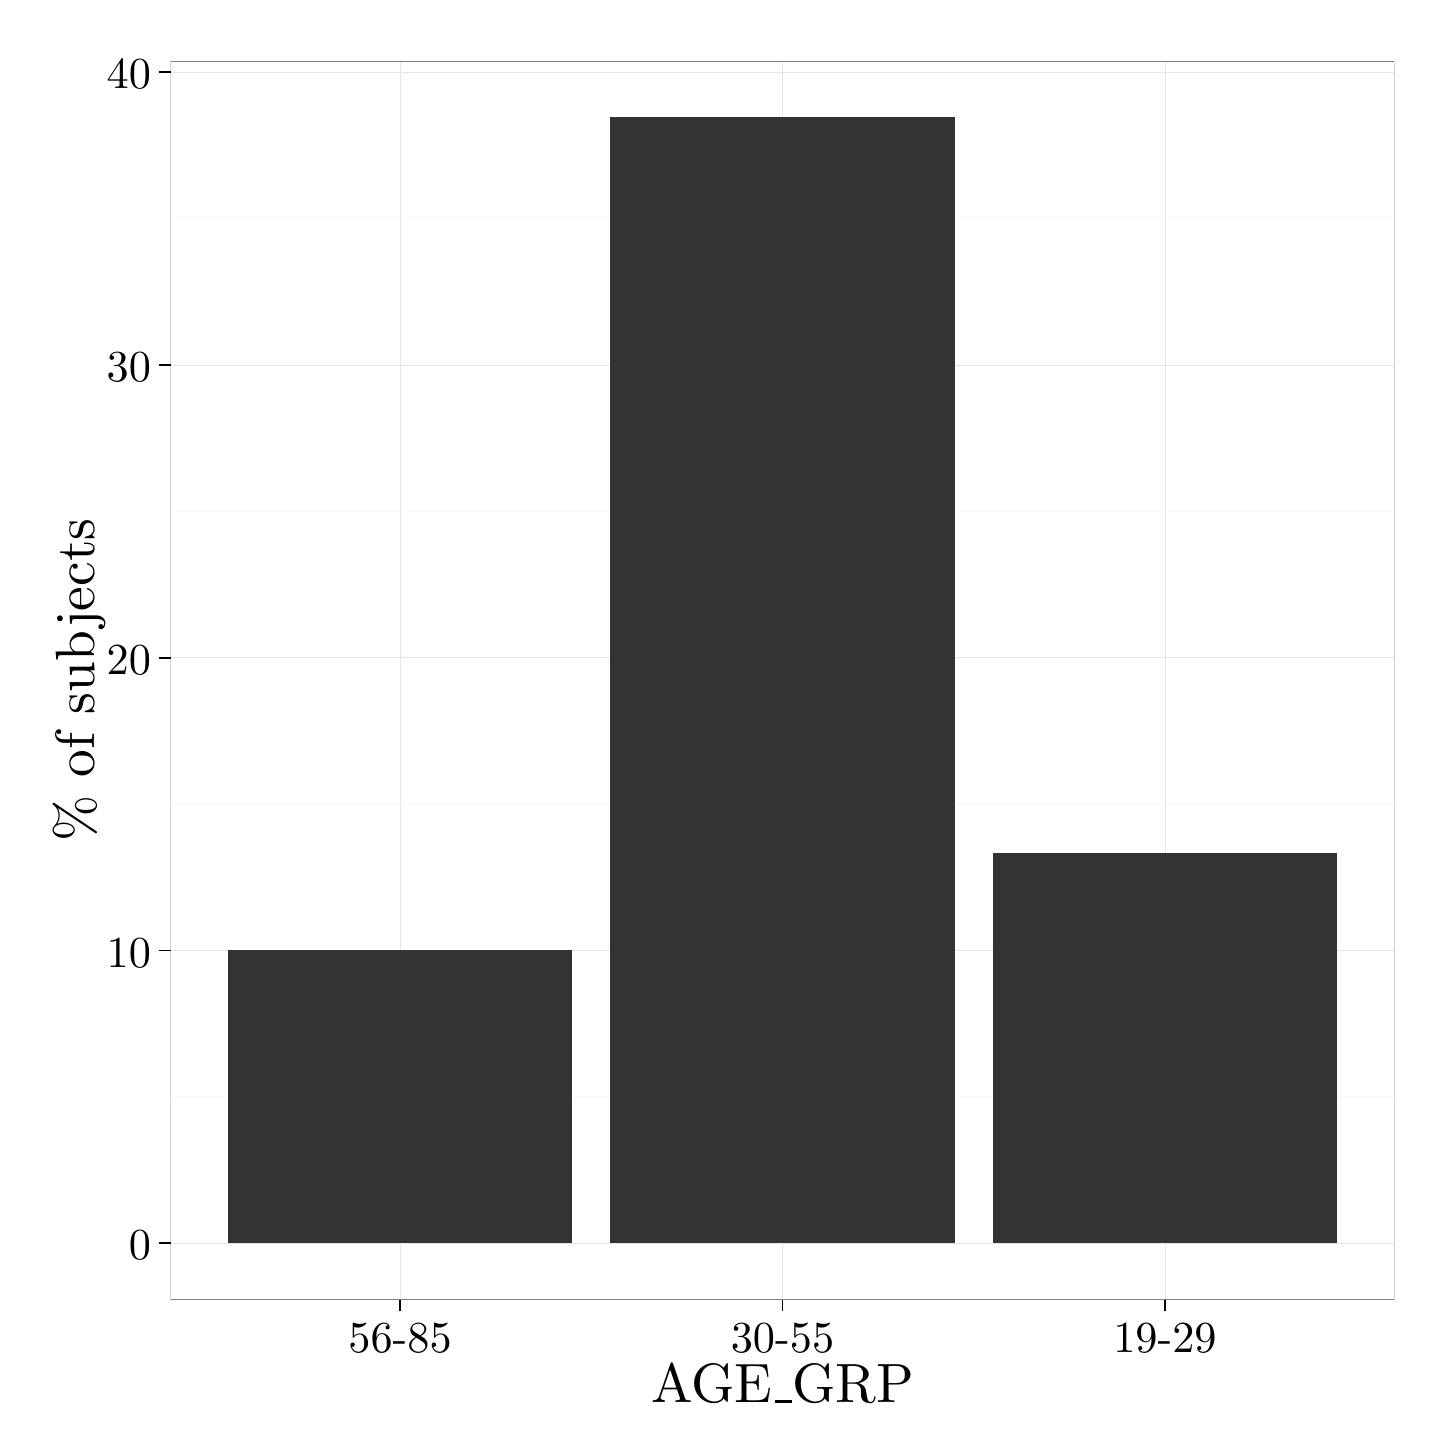
\begin{tikzpicture}[x=1pt,y=1pt]
\definecolor{fillColor}{RGB}{255,255,255}
\path[use as bounding box,fill=fillColor,fill opacity=0.00] (0,0) rectangle (505.89,505.89);
\begin{scope}
\path[clip] (  0.00,  0.00) rectangle (505.89,505.89);
\definecolor{drawColor}{RGB}{255,255,255}
\definecolor{fillColor}{RGB}{255,255,255}

\path[draw=drawColor,line width= 0.6pt,line join=round,line cap=round,fill=fillColor] (  0.00, -0.00) rectangle (505.89,505.89);
\end{scope}
\begin{scope}
\path[clip] ( 51.66, 46.31) rectangle (493.85,493.84);
\definecolor{fillColor}{RGB}{255,255,255}

\path[fill=fillColor] ( 51.66, 46.31) rectangle (493.84,493.84);
\definecolor{drawColor}{gray}{0.98}

\path[draw=drawColor,line width= 0.6pt,line join=round] ( 51.66,119.54) --
	(493.85,119.54);

\path[draw=drawColor,line width= 0.6pt,line join=round] ( 51.66,225.33) --
	(493.85,225.33);

\path[draw=drawColor,line width= 0.6pt,line join=round] ( 51.66,331.11) --
	(493.85,331.11);

\path[draw=drawColor,line width= 0.6pt,line join=round] ( 51.66,436.90) --
	(493.85,436.90);
\definecolor{drawColor}{gray}{0.90}

\path[draw=drawColor,line width= 0.2pt,line join=round] ( 51.66, 66.65) --
	(493.85, 66.65);

\path[draw=drawColor,line width= 0.2pt,line join=round] ( 51.66,172.44) --
	(493.85,172.44);

\path[draw=drawColor,line width= 0.2pt,line join=round] ( 51.66,278.22) --
	(493.85,278.22);

\path[draw=drawColor,line width= 0.2pt,line join=round] ( 51.66,384.01) --
	(493.85,384.01);

\path[draw=drawColor,line width= 0.2pt,line join=round] ( 51.66,489.79) --
	(493.85,489.79);

\path[draw=drawColor,line width= 0.2pt,line join=round] (134.57, 46.31) --
	(134.57,493.84);

\path[draw=drawColor,line width= 0.2pt,line join=round] (272.75, 46.31) --
	(272.75,493.84);

\path[draw=drawColor,line width= 0.2pt,line join=round] (410.94, 46.31) --
	(410.94,493.84);
\definecolor{fillColor}{gray}{0.20}

\path[fill=fillColor] ( 72.39, 66.65) rectangle (196.75,172.44);

\path[fill=fillColor] (210.57, 66.65) rectangle (334.94,473.50);

\path[fill=fillColor] (348.75, 66.65) rectangle (473.12,207.66);
\definecolor{drawColor}{gray}{0.50}

\path[draw=drawColor,line width= 0.6pt,line join=round,line cap=round] ( 51.66, 46.31) rectangle (493.84,493.84);
\end{scope}
\begin{scope}
\path[clip] (  0.00,  0.00) rectangle (505.89,505.89);
\definecolor{drawColor}{RGB}{0,0,0}

\node[text=drawColor,anchor=base east,inner sep=0pt, outer sep=0pt, scale=  1.60] at ( 44.55, 60.62) {0};

\node[text=drawColor,anchor=base east,inner sep=0pt, outer sep=0pt, scale=  1.60] at ( 44.55,166.40) {10};

\node[text=drawColor,anchor=base east,inner sep=0pt, outer sep=0pt, scale=  1.60] at ( 44.55,272.19) {20};

\node[text=drawColor,anchor=base east,inner sep=0pt, outer sep=0pt, scale=  1.60] at ( 44.55,377.97) {30};

\node[text=drawColor,anchor=base east,inner sep=0pt, outer sep=0pt, scale=  1.60] at ( 44.55,483.76) {40};
\end{scope}
\begin{scope}
\path[clip] (  0.00,  0.00) rectangle (505.89,505.89);
\definecolor{drawColor}{RGB}{0,0,0}

\path[draw=drawColor,line width= 0.6pt,line join=round] ( 47.39, 66.65) --
	( 51.66, 66.65);

\path[draw=drawColor,line width= 0.6pt,line join=round] ( 47.39,172.44) --
	( 51.66,172.44);

\path[draw=drawColor,line width= 0.6pt,line join=round] ( 47.39,278.22) --
	( 51.66,278.22);

\path[draw=drawColor,line width= 0.6pt,line join=round] ( 47.39,384.01) --
	( 51.66,384.01);

\path[draw=drawColor,line width= 0.6pt,line join=round] ( 47.39,489.79) --
	( 51.66,489.79);
\end{scope}
\begin{scope}
\path[clip] (  0.00,  0.00) rectangle (505.89,505.89);
\definecolor{drawColor}{RGB}{0,0,0}

\path[draw=drawColor,line width= 0.6pt,line join=round] (134.57, 42.04) --
	(134.57, 46.31);

\path[draw=drawColor,line width= 0.6pt,line join=round] (272.75, 42.04) --
	(272.75, 46.31);

\path[draw=drawColor,line width= 0.6pt,line join=round] (410.94, 42.04) --
	(410.94, 46.31);
\end{scope}
\begin{scope}
\path[clip] (  0.00,  0.00) rectangle (505.89,505.89);
\definecolor{drawColor}{RGB}{0,0,0}

\node[text=drawColor,anchor=base,inner sep=0pt, outer sep=0pt, scale=  1.60] at (134.57, 27.13) {56-85};

\node[text=drawColor,anchor=base,inner sep=0pt, outer sep=0pt, scale=  1.60] at (272.75, 27.13) {30-55};

\node[text=drawColor,anchor=base,inner sep=0pt, outer sep=0pt, scale=  1.60] at (410.94, 27.13) {19-29};
\end{scope}
\begin{scope}
\path[clip] (  0.00,  0.00) rectangle (505.89,505.89);
\definecolor{drawColor}{RGB}{0,0,0}

\node[text=drawColor,anchor=base,inner sep=0pt, outer sep=0pt, scale=  2.00] at (272.75,  9.03) {AGE{\_{}}GRP};
\end{scope}
\begin{scope}
\path[clip] (  0.00,  0.00) rectangle (505.89,505.89);
\definecolor{drawColor}{RGB}{0,0,0}

\node[text=drawColor,rotate= 90.00,anchor=base,inner sep=0pt, outer sep=0pt, scale=  2.00] at ( 24.12,270.08) {{\%} of subjects};
\end{scope}
\end{tikzpicture}
} 
	\caption{Awareness of \textsc{nurse} by age}
	\label{fig.aware.nurse}
\end{figure}

\figref{fig.aware.nurse} summarises aware\is{awareness}ness of the \textsc{nurse}-\textsc{square} merger in the three age groups under scrutiny in this study.
As explained at the beginning of this chapter, the database for this bar plot is not restricted to the 20 interviews used for the quantitative analyses, but includes information extracted from all 38 interviews that have been conducted by the author.
The height of the bars represent the percentages of subjects in the relevant age groups who showed some sort of conscious\is{awareness} aware\is{awareness}ness of the \textsc{nurse}-\textsc{square} merger, i.e. they either gave an explicit explanation of the feature or they at least provided relevant examples.
As is obvious from the left-most bar, only 10\% of the speakers in the oldest group mentioned this feature, so we can say that the variable is virtually unknown in this age group.
In the middle-aged group (bar in the middle), 38.46\% mentioned the feature.
While this means that people who are not conscious\is{awareness}ly aware\is{awareness} of this variable are still in the majority, aware\is{awareness}ness \emph{has} increased considerably and the feature does seem to have acquired a certain degree of \isi{salience} within this group.
When we look at the youngest speakers, however, this trend has apparently not been maintained: the percentage of subjects who explicitly commented on the \textsc{nurse}-\textsc{square} merger has not increased further, but actually dropped again to 13.33\%, a value which is comparable to that of the oldest Liverpudlians in the sample.
With respect to this vowel, therefore, \isi{salience} seems to have decreased in the 19--29 year olds, only a small minority knows that fronted \textsc{nurse} variants are a characteristic feature of Liverpool English.

\subsubsection{Lenition of /k/}
\label{aware_res.phon.k}

As far as lenition is concerned, it is first of all interesting to note that none of the 4 old speakers in the primary sample of this study talk about this feature at all.
The retired teacher quoted at the beginning of \sectref{aware_res.phon} \emph{might} constitute an exception, but even if one is willing to accept her statement as referring to lenition, it would clearly relate to lenition of \emph{alveolar} plosives, not \emph{velar} ones, which are the focus of this research.

In the group of subjects aged between 30 and 55, however, we do find a number of quotes that directly and explicitly refer to the way Scousers realise the phoneme /k/.
Just as with the \textsc{nurse}-\textsc{square} merger, some of these comments are comparatively vague and essentially just consist of an example word containing the relevant variable.
A female working-class speaker in this sub-sample, for instance, explained that one could identify someone from Liverpool based on ``how people say \emph{chicken} and all that'' (13FWC44).
Other speakers explicitly generalise and talk about the variable instead of just single words (``we pronounce `k's quite strongly at the end of words, (\ldots) or within words'' -- 33FMC38), although these more general descriptions are also often backed up with concrete examples (``people used to always ask me to say \emph{chicken}'' -- 33FMC38).
What is more, people often additionally single out the relevant variable (``it's like /x/'' -- 33FMC38) and describe the place of articulation, phonetically correctly, as ``like, (quite) guttural, isn't it'' (33FMC38 and 01MMC52).

If we focus on the youngest Liverpudlians that have been interviewed, explicit comments\is{overt commentary} on lenition of /k/ actually abound -- each of the 8 subjects in this age group that were included in the quantitative analysis mentioned this variable.
Again, there are some rather vague explanations, such as one 19-year-old middle-class male referring to lenition of velar plosives as Liverpudlians ``put[ting] an emphasis on `k's'' (31MMC19).
Most other comments in this age group, however, are very much to the point.
One speaker mentions the variable (``definitely the ``k''), provides examples (``if I was to say (\ldots) \emph{cook} [kʊx], \emph{back} [bax]''), contrasts the standard realisation with the Scouse one, and even talks about his difficulties in producing the former: 
\begin{example}
	It's really hard for me to say [tʊk] rather than [tʊx]. (02MWC20)
\end{example}

These speakers are also aware\is{awareness} of the fact that the ``/x/ at the back of your throat'' is particularly frequent in ``some of the strong accents'' and ``quite distinct\is{distinctness}ive'' as well (04MWC19).
Another subject in this age group even declares lenition of velar plosives to be a \isi{shibboleth}.
When asked to name sounds that distinguish Liverpool English from other accents he says:
\begin{example}
	Of course you can tell (\ldots) if people have the /x/ sound (\ldots) when they speak.
	So it's easy to tell who's a Scouser\is{identity}, and who's not a Scouser\is{identity}. (25MMC19)
\end{example}
Other Liverpudlians between the ages of 19 and 29 also count ``the /x/ sound'' among the ``main, like, characteristics of the accent'' (36FWC20).
This does not necessarily mean that they like this feature, though.
For example, a middle-class female who talks about the ``throaty /x/'' in words like \emph{chicken} and \emph{bucket} also explains that she finds this pronunciation ``really annoying'' (06FMC20).

It is not unlikely that younger Scousers are particularly aware\is{awareness} of this variable because it is not just a \isi{shibboleth} for Liverpudlians, but also for outsiders.
Two speakers in the sample mention lenition of /k/ as a typical feature of Scouse and reveal that their judgement is not exclusively influenced by their own observations, but, at least in part, by external perceptions of Liverpool English as well.
Both are working-class women and 20 years old.
The first one names ``the /x/ sound'' as a typical Scouse pronunciation variant and adds that this statement is ``based on what [she's] been skitted on in the past'' (36FWC20), so she is especially conscious\is{awareness} of the feature because other people (who are, presumably, not from Liverpool) have used it to make fun of her.
The second speaker also provides a personal mini-narrative when she recounts that ``people say `say chicken', 'cause we say [t͡ʃɪxən]'', and that ever since she entered university she had frequently been asked ``do you want some chicken?'' by people who wanted to ``imitate [her]'' (37FWC20).
It is well possible that many other Liverpudlians have made rather similar experiences when interacting with speakers from other areas.
After all, lenition is not only classified as a highly characteristic feature of Scouse by linguists, but, impressionistically at least, it also seems to be omnipresent in all imitation\is{accent performance}s of Scouse by stand-up comedians and the like.

\begin{figure}[h]
	\centering
		\definecolor{shadecolor}{rgb}{0.969, 0.969, 0.969}
		\resizebox{.49\linewidth}{!}{% Created by tikzDevice version 0.8.1 on 2016-02-09 02:17:46
% !TEX encoding = UTF-8 Unicode
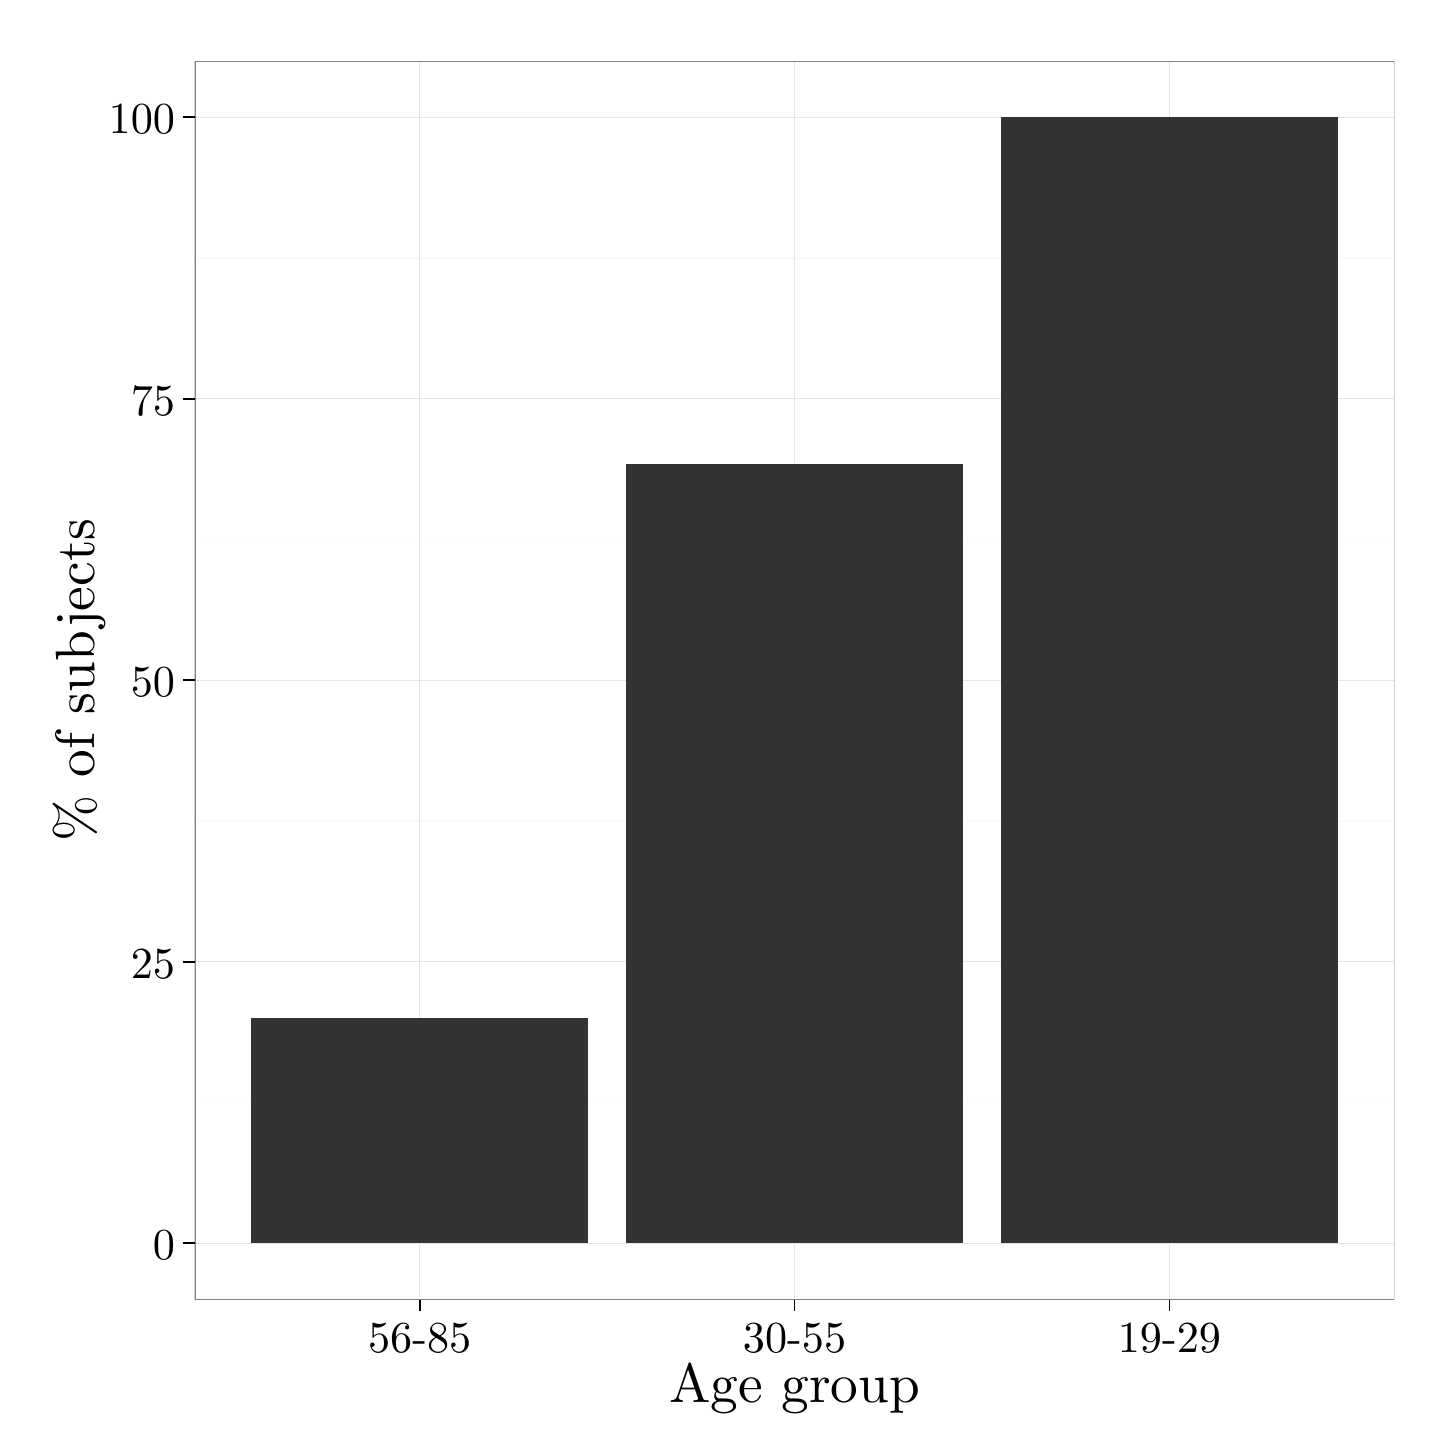
\begin{tikzpicture}[x=1pt,y=1pt]
\definecolor{fillColor}{RGB}{255,255,255}
\path[use as bounding box,fill=fillColor,fill opacity=0.00] (0,0) rectangle (505.89,505.89);
\begin{scope}
\path[clip] (  0.00,  0.00) rectangle (505.89,505.89);
\definecolor{drawColor}{RGB}{255,255,255}
\definecolor{fillColor}{RGB}{255,255,255}

\path[draw=drawColor,line width= 0.6pt,line join=round,line cap=round,fill=fillColor] (  0.00, -0.00) rectangle (505.89,505.89);
\end{scope}
\begin{scope}
\path[clip] ( 60.37, 46.31) rectangle (493.85,493.84);
\definecolor{fillColor}{RGB}{255,255,255}

\path[fill=fillColor] ( 60.37, 46.31) rectangle (493.85,493.84);
\definecolor{drawColor}{gray}{0.98}

\path[draw=drawColor,line width= 0.6pt,line join=round] ( 60.37,117.51) --
	(493.85,117.51);

\path[draw=drawColor,line width= 0.6pt,line join=round] ( 60.37,219.22) --
	(493.85,219.22);

\path[draw=drawColor,line width= 0.6pt,line join=round] ( 60.37,320.93) --
	(493.85,320.93);

\path[draw=drawColor,line width= 0.6pt,line join=round] ( 60.37,422.65) --
	(493.85,422.65);
\definecolor{drawColor}{gray}{0.90}

\path[draw=drawColor,line width= 0.2pt,line join=round] ( 60.37, 66.65) --
	(493.85, 66.65);

\path[draw=drawColor,line width= 0.2pt,line join=round] ( 60.37,168.36) --
	(493.85,168.36);

\path[draw=drawColor,line width= 0.2pt,line join=round] ( 60.37,270.08) --
	(493.85,270.08);

\path[draw=drawColor,line width= 0.2pt,line join=round] ( 60.37,371.79) --
	(493.85,371.79);

\path[draw=drawColor,line width= 0.2pt,line join=round] ( 60.37,473.50) --
	(493.85,473.50);

\path[draw=drawColor,line width= 0.2pt,line join=round] (141.65, 46.31) --
	(141.65,493.84);

\path[draw=drawColor,line width= 0.2pt,line join=round] (277.11, 46.31) --
	(277.11,493.84);

\path[draw=drawColor,line width= 0.2pt,line join=round] (412.57, 46.31) --
	(412.57,493.84);
\definecolor{fillColor}{gray}{0.20}

\path[fill=fillColor] ( 80.69, 66.65) rectangle (202.61,148.02);

\path[fill=fillColor] (216.15, 66.65) rectangle (338.07,348.31);

\path[fill=fillColor] (351.61, 66.65) rectangle (473.53,473.50);
\definecolor{drawColor}{gray}{0.50}

\path[draw=drawColor,line width= 0.6pt,line join=round,line cap=round] ( 60.37, 46.31) rectangle (493.85,493.84);
\end{scope}
\begin{scope}
\path[clip] (  0.00,  0.00) rectangle (505.89,505.89);
\definecolor{drawColor}{RGB}{0,0,0}

\node[text=drawColor,anchor=base east,inner sep=0pt, outer sep=0pt, scale=  1.60] at ( 53.26, 60.62) {0};

\node[text=drawColor,anchor=base east,inner sep=0pt, outer sep=0pt, scale=  1.60] at ( 53.26,162.33) {25};

\node[text=drawColor,anchor=base east,inner sep=0pt, outer sep=0pt, scale=  1.60] at ( 53.26,264.04) {50};

\node[text=drawColor,anchor=base east,inner sep=0pt, outer sep=0pt, scale=  1.60] at ( 53.26,365.76) {75};

\node[text=drawColor,anchor=base east,inner sep=0pt, outer sep=0pt, scale=  1.60] at ( 53.26,467.47) {100};
\end{scope}
\begin{scope}
\path[clip] (  0.00,  0.00) rectangle (505.89,505.89);
\definecolor{drawColor}{RGB}{0,0,0}

\path[draw=drawColor,line width= 0.6pt,line join=round] ( 56.10, 66.65) --
	( 60.37, 66.65);

\path[draw=drawColor,line width= 0.6pt,line join=round] ( 56.10,168.36) --
	( 60.37,168.36);

\path[draw=drawColor,line width= 0.6pt,line join=round] ( 56.10,270.08) --
	( 60.37,270.08);

\path[draw=drawColor,line width= 0.6pt,line join=round] ( 56.10,371.79) --
	( 60.37,371.79);

\path[draw=drawColor,line width= 0.6pt,line join=round] ( 56.10,473.50) --
	( 60.37,473.50);
\end{scope}
\begin{scope}
\path[clip] (  0.00,  0.00) rectangle (505.89,505.89);
\definecolor{drawColor}{RGB}{0,0,0}

\path[draw=drawColor,line width= 0.6pt,line join=round] (141.65, 42.04) --
	(141.65, 46.31);

\path[draw=drawColor,line width= 0.6pt,line join=round] (277.11, 42.04) --
	(277.11, 46.31);

\path[draw=drawColor,line width= 0.6pt,line join=round] (412.57, 42.04) --
	(412.57, 46.31);
\end{scope}
\begin{scope}
\path[clip] (  0.00,  0.00) rectangle (505.89,505.89);
\definecolor{drawColor}{RGB}{0,0,0}

\node[text=drawColor,anchor=base,inner sep=0pt, outer sep=0pt, scale=  1.60] at (141.65, 27.13) {56-85};

\node[text=drawColor,anchor=base,inner sep=0pt, outer sep=0pt, scale=  1.60] at (277.11, 27.13) {30-55};

\node[text=drawColor,anchor=base,inner sep=0pt, outer sep=0pt, scale=  1.60] at (412.57, 27.13) {19-29};
\end{scope}
\begin{scope}
\path[clip] (  0.00,  0.00) rectangle (505.89,505.89);
\definecolor{drawColor}{RGB}{0,0,0}

\node[text=drawColor,anchor=base,inner sep=0pt, outer sep=0pt, scale=  2.00] at (277.11,  9.03) {Age group};
\end{scope}
\begin{scope}
\path[clip] (  0.00,  0.00) rectangle (505.89,505.89);
\definecolor{drawColor}{RGB}{0,0,0}

\node[text=drawColor,rotate= 90.00,anchor=base,inner sep=0pt, outer sep=0pt, scale=  2.00] at ( 24.12,270.08) {{\%} of subjects};
\end{scope}
\end{tikzpicture}
} 
	\caption{Awareness of /k/ lenition by age}
	\label{fig.aware.k}
\end{figure}

If we again zoom out a bit further and take into account all 38 interviews, the picture sketched above solidifies.
Just as for the \textsc{nurse}-\textsc{square} merger, \figref{fig.aware.k} shows the percentage of speakers in the relevant age group that explicitly mentioned lenition of /k/ as a typical feature of Scouse.
As can be seen quite clearly, the rate is, at 20\%, quite low in the oldest group of speakers, which is represented by the bar on the left of the graph.
Only one in five speakers aged 56 and older commented on lenition.
In the middle-aged group, this rate has risen quite considerably: almost three out of four subjects (69.23\%) are now aware\is{awareness} of lenited /k/ variants.
When we finally get to the youngest speakers investigated in this study, the bar (on the right) in the plot actually reaches the 100\% threshold, which means that \emph{every single} participant under 30 explicitly mentioned lenition of velar plosives as a typical feature of Scouse and commented on it.
Awareness of lenition thus increases in a near-linear fashion from the oldest to the youngest participants: it starts out as a feature which only a handful of Liverpudlians are aware\is{awareness} of, gains dramatically in prominence in the middle group, and finally reaches a state of full conscious\is{awareness} aware\is{awareness}ness in the youngest generation of speakers interviewed.

Having said all that, it should be noted that it is quite possible that Scousers are \emph{generally} aware\is{awareness} of the variable but not, for some reason, of its presence \emph{in their own speech}\is{linguistic insecurity}.
There is some anecdotal evidence in my data that supports this idea.
One subject (female, working-class, 20 years old) explicitly said that she didn't like lenition and therefore didn't use it:
\begin{example}
	I can't even do it because I've spent that long, trying to, like, train me mouth not to do it. (36FWC20)
\end{example}
However, she has a mean \isi{PDF} of 81.87\%.
So in actual fact, she \emph{can} do it quite well, and uses the fricative realisation almost categorically.
Very similar things could probably be said about a number of other subjects who proclaimed not to have a strong Scouse accent or who said they did not like lenited /k/ variants, but who nevertheless quite frequently \emph{use} these variants.

\section{Evolution and evaluation of Scouse}
\label{aware_res.eval}

\subsection{Old speakers}
\label{aware_res.eval.old}

\subsubsection{Increase of `slovenly Scouse'}
\label{aware_res.eval.old.change}

All four older subjects in the primary sample in one way or another express the idea that Scouse has ``really \isi{change}d in the younger generation'' (28FMC59).
Two of them make reference to the Beatles, whose ``Liverpool accent'' was allegedly ``different (\ldots) because (\ldots) it's become very guttural now'' (08MMC62).
One might be tempted to interpret this statement as referring to increased usage of the `guttural' /k/ lenition (cf. \sectref{sec.prod.res.con.k.agegender}), and this might very well be what the speaker is talking about.
However, the same term is also used by a female subject of about the same age when she says that ``it used to be (\ldots) quite guttural, the way \emph{we} spoke'' (28FMC59, my emphasis).
It follows that, for her, Scouse has thus become \emph{less} `guttural'.
This could either mean she has not noticed that younger Liverpudlians use more lenition, or that she thinks of something completely different when she says `guttural'.
In any case, she seems to think that Liverpool English has become more distinct\is{distinctness} from the surrounding area in her life time, because she explains that in the accent she ``grew up with in the sixties, that everybody recognised through the Beatles'', one encountered ``\isi{Lancashire} expressions very often'' (28FMC59).
She believes ``the older accent'' can still be heard in ``[her] generation and the older people'', whereas her sons could ``perfectly mimic young Scouse men talking now'' which apparently sounds ``just bizarre'' and ``strange'' because the accent has ``really, really \isi{change}d'' (28FMC59).

Another speaker has the impression that ``the percentage of people that speak really slovenly Scouse has increased'' (05MWC66).
This \isi{change} is, in his opinion, primarily driven by ``the poorer people'', but he also finds that ``it's mostly young people that talk like that'', presumably because ``as they get older (\ldots) [their accent] gets a bit rounded off (05MWC66).
If we follow this line of argumentation, the increase of `slovenly Scouse' would only be temporary on the level of the individual and restricted to speakers of a certain age (the same at any point in time!) at the level of the \isi{speech community}.
In opposition to this, another speaker states that the present generation``has got it's own language'' in much the same way as ``[her] generation had a language that was different from our parents''', so she seems to find it quite natural that ``each generation just create[s] their own language completely'' (18FWC67) -- without suggesting that this is something that people necessarily do away with later in their life.

While this is a rather liberal stance on language \isi{change}, it does not completely keep her from seeing something special in the most recent \isi{change}s that she does not seem to be too happy about.
According to her, ``there are youngsters that will (\ldots) not say the words properly and they will put (\ldots) the Scouse accent on'' (18FWC67).
While it is not quite clear what exactly she means by `not saying the words properly', it is probably uncontroversial to assume she is referring to non-standard pronunciation, coupled with the fact that this seems to happen in a non-natural, inauthentic\is{authenticity} way, as the second part of the quote suggests. This `putting it on' is something she observes in her own family (``grandson can do it very well''), and which, apparently, can start with children that are ``only nine'' (18FWC67).
Not only does she believe that the variety that younger Liverpudlians use is ``totally different from the language [she] had, and [her] daughter had'', but she even maintains that her two grandsons differed in linguistic behaviour, despite the fact that ``there's only two years between the two of them'' (18FWC67).
Both, however, seem to be using varieties of English that are considerably different from her own because she reports frequently having to ask both of them to repeat utterances she did not understand.

This subject and the other woman in the group of older speakers hint at a possible reason why the accents of young Liverpudlians seem particularly strong to this generation.
When (presumably) talking about the \textsc{nurse}-\textsc{square} merger (cf. \sectref{aware_res.phon}) she does not only mention that younger Scousers `keep their teeth together' but she also adds that speakers of her generation ``weren't allowed to do that'' and that they ``got told off'' if they spoke with a markedly non-standard accent (18FWC67).
The newly-retired teacher gives a slightly more detailed account and explains that her accent is now ``modified (\ldots), probably 'cause we had elocution at school'' (28FMC59).
Further research would be required to analyse if this is an experience that is rather particular to this individual speaker because she was ``educated by nuns'' and later became a teacher, or whether a sizeable proportion of Liverpudlians in this generation ``learned to speak a more received pronunciation'' (28FMC59) during their time at school.

\subsubsection{From `amiable' to `grating'}
\label{aware_res.eval.old.like}

When it comes to the evaluation of this \isi{change}, the older speakers in my sample are relatively unanimous.
The male working-class subject links stronger accents up not just with youth, but also with social deprivation when he says that ``it's not all young people that talk like that'', but especially ``the poorer [ones]'' among them; a fact which he does not ``decry[]'' but which he attributes to the influence of their peers (05MWC66).
He adds that he knows he himself speaks with a Scouse accent, but -- crucially -- ``people can understand [him]'' (05MWC66).
The value judgement is not explicit here, but nevertheless not too difficult to unearth: he does not object to Scouse accents in general, as long as they do not hinder communication.
A mild accent that expresses where one is from is fine, a strong one which makes it difficult (for outsiders) to understand the speaker, is not.
His middle-class counterpart essentially voices the same belief, but does so in a more direct way.
In his opinion, the accent has ``got a lot coarser'' and ``harder (\ldots) amongst younger people'' (08MMC62).
His choice of vocabulary already clearly suggests that he considers this to be ``not so good'', but his main criticism is that the supposed coarseness can ``make [younger Scousers] unintelligible\is{unintelligibility}, (\ldots) and they don't have to be'' (08MMC62).
It does not take too much interpretation to arrive at the conclusion that he probably also thinks they \emph{should} not be.

Unintelligibility is, however, not the only potential problem that this age group sees in pronounced Liverpool accents.
The working-class male explains that, for him, strong Scouse accents are ``normal'' because he has grown up in the city, but he also finds it understandable that ``the way some [Scousers] (\ldots) talk (\ldots) can be intimidating'' to \emph{outsiders} (05MWC66).
According to him, the ``very, very few'' Liverpudlians who use these strong accents do not ``do good for us'' (05MWC66), i.e. they have a detrimental influence on the national \isi{image} of Liverpool because, with their strong and `intimidating' accents, they give an impression of the city which people from outside find rather unpleasant.
This speaker is not exclusively worried about external perceptions, though, but also states that he himself is not a fan of `slovenly Scouse' -- as he calls it --, when he reflects about people's motivation for using these varieties: 
\begin{example}
	I don't think they've conscious\is{awareness}ly gone out to say `we'll speak this way so to get on everybody's nerves'. The fact that it does is a bonus. (05MWC66)
\end{example}
So, while he does not assume that young Scousers \emph{primarily} employ strong accents to annoy other people, he does believe that they like the idea (`a bonus') and he also acknowledges that they have this effect on him personally (`the fact that it does').

The two women in this age group seem to largely agree with this evaluation.
One of them states that ``the ordinary Scouse is quite amiable'', but ``the really (\ldots) guttural one that they used in \emph{Bread} (\ldots) grates on your nerves'' (18FWC67).
Strong accents, such as the one that is heard in the BBC sitcom from the 80s, `grate', in her opinion, ``because there's only a certain community that talks like that'' (18FWC67) -- presumably very deprived and poor people like the fictitious lower working-class family which \emph{Bread} revolves around.
While she does not claim that these kinds of accents are \emph{exclusively} found among younger Liverpudlians, she does stress that particularly ``some youngsters'' use a kind of ``plucking chicken language'' (18FWC67), an attribute which can hardly be considered positive.
The other older female speaker gives a very similar verdict when she says that, to her, modern Scouse accents seem ``more staccato'' than they used to be (28FMC59).
She is not really happy about this and finds the resulting sound ``not gentle'' and ``much more aggressive'' (28FMC59) than the one she considers typical of her own youth.

\subsection{Middle-aged speakers}
\label{aware_res.eval.mid}

\subsubsection{Kids so Scouse it's unbelievable}
\label{aware_res.eval.mid.change}

In the middle-aged group, fewer subjects explicitly talk about \isi{change} in Liverpool English, but when they do their gist is similar to that of the oldest speakers in the sample.
A male, middle-class speaker, for instance, argues there is `no doubt about it'' that Scouse ``definitely has \isi{change}d'' and he even provides a quite precise estimate that this is something that has happened in the ``last sort of 10 years'' (01MMC52).
He also says that ``when [he] was young'' the accent was allegedly more ``lyrical'' and ``singy songy'', something which, he explains, can also still be heard in the speech of ``some of the older people'', so this is further evidence for the fact that he believes \isi{change} in Scouse to be a rather new development, ``something that's recently cracked in'' (01MMC52).
The same speaker also brings up the issue of \isi{unintelligibility}, although he does not directly link it to younger Liverpudlians.
He refers to an acquaintance who has ``a really thick accent'' and who, on a particular occasion, spoke in a way which made it impossible for a friend from Staffordshire to ``understand him at all'' (01MMC52).
He goes on to explain that this was, in his opinion, mostly due to lenition of velar plosives (``he does /x/'') and that he also believes that ``he embellishes [his accent]'' and ``lay[s] it on a lot'' (01MMC52), so a very strong accent that is unintelligible\is{unintelligibility} (to outsiders) is once more associated with inauthentic\is{authenticity}ity.

Other speakers in this age group connect these kinds of accents more directly and explicitly with young Scousers.
A 49-year-old working-class male\footnote{During the interview of this subject the recording equipment failed. As a result, the last 2 minutes or so of his interview were not recorded. The above reproduction of his relevant statements is based on notes taken directly after the interview.}, for instance, claimed that the accent was getting stronger and `rougher' with younger speakers, while not bringing up the subject of \isi{unintelligibility}.
One of his female counterparts, however, does just that in the following statement:
\begin{example}
	The kids, you know, they're so Scouse it's unbelievable. (\ldots) I have difficulty understanding some of them. (13FWC44)
\end{example}
Here, the matter of \isi{change} and \isi{unintelligibility} is taken one step further.
For this particular speaker, it is no longer just an issue of young Scousers being unintelligible\is{unintelligibility} to people who are not familiar with Liverpool accents.
When she says that she herself sometimes has to ``ask [her nieces and nephews] twice what they're saying'' (13FWC44) she acknowledges that even middle-aged insiders occasionally run into difficulties when talking to young Liverpudlians with pronounced local accents.
Interestingly, she also hypothesises about whether this might be a temporary issue, i.e. whether younger speakers might \isi{change} their pronunciation to a more standard-like (or at least less local) accent later in their life (cf. \sectref{aware_res.eval.old}).
Her argument for this idea is based on pragmatic and presumably also economic and social reasons, because she explains that ``as you get older and you're getting to work (\ldots), you have to tone [the accent] down'', and adds that this is particularly true ``when you're dealing with the public'' (13FWC44) -- in cases where the speaker is in an exposed position where both intelligibility and social appropriateness are an issue.

\subsubsection{From `down-to earth' to `thick'}
\label{aware_res.eval.mid.like}

Middle-aged speakers evaluate Scouse and the perceived \isi{change} in the accent in a very similar way as the oldest subjects do (cf. \sectref{aware_res.eval.old.like}).
There is only one speaker in this age group who has exclusively positive things to say about Scouse.
This woman explains that ``[she] quite like[s] the accent'', because for her ``it sounds friendly'' and ``down to earth'' (33FMC38).
She also says that it does not sound ``stuck up'' (33FMC38), thereby implying that other varieties do, but without specifying which ones precisely she is comparing Scouse to.
Other speakers focus more on negative aspects: the working-class male who classified the accents of younger Scousers as being `rougher', for instance, also explained that he found these accents `unpleasant' (17MWC49), a judgement which is already implicit in a term like `rough'.

This speaker, and some others likewise, only explicitly talk about aspects of Scouse that they find disagreeable, but by expressly limiting their statements to particular sub-variants of Scouse (i.e. `strong' ones) they also imply that they evaluate other (`lighter') accents differently.
For instance, the 52-year-old male in the sample is only talking about particularly strong Scouse accents as they are, in his opinion often found in younger speakers when he says: ``I don't like it, no. I just kind of think it's a bit put on'' (01MMC52).
It should be noted that the dislike is, once more, connected with the fact that these accents are perceived as inauthentic\is{authenticity} and ``false'' (01MMC52).

Some subjects in this age group do, however, explicitly contrast different varieties of Scouse and make clear that they also judge them differently.
One working-class woman, for example, says that  she ``[doesn't] like the \emph{broad} Scouse'' because ``it can sound thick, like somebody's not all together there'', whereas speaking ``with a little twang is alright'' (13FWC44, my emphasis).
In this particular case, `sounding thick' seems to be somewhat intermingled with communicative problems, because the subject immediately follows up the above statement with (another) short narrative of her nephew who apparently often talks in a way that ``you just can't understand a word he's saying'', so ``he certainly couldn't communicate with an adult'' but only ``with his mates'' and should therefore ``tone it down a bit'' (13FWC44).
It is possible that this line of thought is limited to this one individual, but it would not be surprising if `being unintelligible\is{unintelligibility}' and `sounding unintelligent' turned out to be related concepts for many other speakers as well.

The following quote from a 33-year-old middle-class male probably quite nicely sums up \isi{attitude}s towards Scouse in this age group:
\begin{example}
	I think a natural sounding Liverpool accent that's not affected in any way sounds very nice, you know.
	I think, unfortunately, these days, there is an element of affectation.
	I think, again, probably that's just young people generally, you know.
	(\ldots) I like the lilt, too [of the unaffected accent].
	I like the (\ldots) character that it brings.
	I don't like the over-emphasis of certain traits within the accent. (03MMC33)
\end{example}

Softer accents bring character and are perceived as nice, pleasant, and agreeable.
Very pronounced accents, however, are not.
The distinction into stronger and lighter accents is not expressly made in this quote, but it is paraphrased as `over-emphasis', on the one hand, and `unaffected' and `natural', on the other.
It seems to me that this is a mental connection which is real for most speakers in this age group, and the old subjects as well.
Strong Scouse accents are not only less acceptable because they can make a speaker unintelligible\is{unintelligibility} (although this does seem to be an important aspect), but also (and maybe even primarily) because middle-aged speakers perceive them as artificial, `affected', and `false'.
From the point of view of my subjects, these accents do make use of features that are recognised as being ``to an extent a part of the accent'' but, crucially, they  are ``overplayed'' (03MMC33), which results in something that is perceived as a stereotypical\is{stereotype} accent perform\is{accent performance}ance and therefore rejected.
While not limited to young Liverpudlians, this group of speakers seems to be the one that my middle-aged subjects primarily associate these `false' accents with.

\subsection{Young speakers}

\subsubsection{A matter of personal experience}
\label{aware_res.eval.young.change}

The speakers aged between 19 and 29 are considerably less homogeneous as a group when it comes to the question of whether Scouse has \isi{change}d or is currently changing.
Some of them, like a 19-year-old working-class male, claim that they have ``not noticed any \isi{change}'' and/or have ``never heard anyone comment the fact the accent's changing at all'', but acknowledge that this might simply be due to their young age and that, for instance, their parents ``might notice differences'' that they themselves do not (04MWC19).
Interestingly however, this speaker then goes on to explain that he would be reluctant to say his own parents ``speak with a Liverpool accent in actual fact'', and that his mother in particular uses ``a softer (\ldots) [and] slightly more refined'' accent (04MWC19).
His personal experience would thus seem to contradict his statement that he has not noticed any \isi{change} in the accent, but apparently he is unwilling to extrapolate the differences within his family to a larger part of the population, for some reason.

The two young middle-class women in the primary sample are very similar in this respect.
When directly asked whether she believes Scouse is changing the first one flatly rejects this idea with the words: ``no, it's about the same'' (06FMC20).
Earlier in her interview, however, when the subject of (local) \isi{identity} was discussed, she explained that she would not use the label `Scouser\is{identity}' for herself, but that she would ``call [her] mum and dad Scouser\is{identity}s, 'cause their accent is significantly stronger than what [hers] is'' (06FMC20).
We have thus, again, a young speaker who has personal experience of \isi{apparent time} \isi{change} (though in the opposite direction of what most older subjects report), but does not seem to consider it representative of the more general situation in Liverpool.

The other female middle-class speaker likewise says that she has not ``noticed [Scouse] changing'', but then immediately goes on to talk about her parents, who ``don't really have a strong Liverpool accent \emph{anymore}'' (my emphasis), despite the fact that they have grown up in the Dingle and Toxteth, respectively, which are both traditional working-class districts that the subject herself describes as ``quite rough areas of Liverpool'', at least when her parents were young (07FMC23).
Her explanation for the `softer' accents of her parents is that they later moved ``out of the centre'' to a northern suburb and ``lost their accent, if they had one'' (07FMC23).
To be fair, the second part of this statement (``if they had one'') indicates that she is aware\is{awareness} of the fact that her parents might never have had such a strong accent as is nowadays typical for speakers from these districts (which would be evidence for accent \isi{change}), but she does not know and apparently prefers the hypothesis that her parents \isi{change}d, instead of the accent itself.
It is possible that this focus on the individual is due to the fact that she has observed \isi{change}s in her own use of language in her recent past.
She speculates that she might have had ``a stronger accent'' before she went to university where she ``lived with quite a lot of people from down south (\ldots) and [her] accent just became really weird'', whereas now that she has been living and working in Liverpool again for a number of years, friends and acquaintances from outside the city tell her that she has ``got more Scouse'' again, though she herself ``can't tell'' (07FMC23).

Most of the subjects that do believe Scouse is changing or has \isi{change}d also base their opinion on evidence collected in their family context.
There is one male middle-class speaker in my sample who believes, and explicitly verbalises, that Liverpool English is ``getting less distinguished'', based on the evidence that in the generation of his grand parents ``they've got really strong accents'' (25MMC19), although it is unclear whether he is primarily referring to his own grand parents or to this age group more generally.
The remainder of the young Scousers, however, agree with the majority of the old and middle-aged speakers in saying that
\begin{inparaenum}[(a)]
	\item ``the accent itself has \isi{change}d, definitely'' (02MWC20), and that
	\item the ``Scouse accent's become stronger'' (31MMC19).
\end{inparaenum}
Younger speakers apparently often realise this first when they compare their own speech with that of other family members, like the middle-class male just quoted, who explains:
\begin{example}
	I talk a bit different to me mum or the rest of me family, but me and me brother talk the same, like, as each other or me mates. (31MMC19)
\end{example}

Some speakers are also conscious\is{awareness} of the fact that there is probably an interaction of age and other social factors like the socioeconomic background of speakers in certain areas of the city.
One interviewee, for instance, says that, in general, Scouse has ``become thicker in a lot of terms'' and adds that this is particularly true in ``deprived areas'' of Liverpool, ``to the point where people (\ldots) have actually asked (\ldots): `Are you from Liverpool?''', despite the fact that he himself has ``a much more heavier accent'' than both his parents (02MWC20).
Another participant provides examples for this claim when she says that ``if you grew up in Anfield or Kensington [inner city working-class districts], you're gonna sound Scouser\is{identity} than someone who grew up in Childwall [a more affluent suburb]'' (36FWC20).
She does, however, also believe that Liverpool English, as a whole, is different today than it was ``a few decades ago'' when it was presumably ``closer to the Manchester accent'' (36FWC20).
Her point of reference seems to be the 60s because she mentions that in ``clips of the Beatles, if you listen to John Lennon speak, he doesn't sound Scouse'' although he was, which is evidence for her that the accent has ``definitely \isi{change}d since then, it's obviously evolved'' (36FWC20).

\subsubsection{`Unpleasant but friendly'}
\label{aware_res.eval.young.like}

With respect to evaluating the perceived \isi{change} of Scouse and its current form, there is again a wide range of different comments and \isi{attitude}s among the youngest speakers in my sample.
Few people directly comment the \isi{change} itself, and when they do they do not express very strong opinions about it.
A male working-class speaker, for instance, says that he ``wouldn't really have a bad or positive comment on the \isi{change}, to be honest'' because for him it is just something that ``happens'' (02MWC20).
A female of the same age explains that she is not sure ``if [she] prefer[s], like, John Lennon's accent to [the modern one]'' or the other way round (36FWC20).
In general, subjects are much more willing to provide evaluations of (varieties of) modern Scouse, rather than on the process of accent \isi{change}.
Often, these judgements are similarly ambiguous as the ones expressed by the old and the middle-aged speakers.
For instance, Scouse can be described as ``unpleasant but (\ldots) friendly at the same time'' because Scouser\is{identity}s are both ``so loud and confident'' (31MMC19).
Another speaker explains that, to him as an insider, ``it sounds friendly, but [he doesn't] know what it sounds, like, from outside looking in'' and he can well imagine that, in the latter case, ``it could be a bit intimidating sometimes'' (25MMC19) -- which is particularly interesting because it is an almost word-by-word repetition of something another Liverpudlians said who is more than 45 years older and from a different social class (cf. \sectref{aware_res.eval.old.like}).

Just like speakers of their parents' and grand parents' generation, the youngest subjects in my sample also often evaluate Scouse differently depending on whether it is considered to be a stronger or a lighter variant.
This is exemplified by statements such as ``if it's a soft Scouse accent (\ldots) I haven't got a problem with it'', provided people ``speak correctly'' and ``as long as I can understand them'' (06FMC20), which is evidence for the fact that (un)intelligibility is as much of an issue and a relevant factor for evaluation among the youngest Scousers as it is in the middle-aged and the old group.
Not every kind of Scouse accent is seen as somewhat problematic, but ``the really, really thick accent where you can't understand what they're saying'' is very frequently, albeit not always, considered as ``very annoying'' (04MWC19).
The same holds true for the whole matter of authentic\is{authenticity}ity.
Consider the following quote:
\begin{example}
	{}[Scouse] does sound quite friendly and I quite like it, unless it's incredibly thick.
	I mean, I like the light accent, and my accent, most Liverpudlian\is{identity} accent[s].
	But when you get over the top with it then it's just plain ridiculous.
	I mean, there's no reason to go /x/ all the time. (04MWC19)
\end{example}
`Thick' accents are judged just as negatively as inauthentic\is{authenticity} ones where people `go over the top with it'.
The `plain ridiculous' accent of this kind is interpreted as the result of a (perhaps semi-)conscious\is{awareness} process, not as something that is just naturally there from the start: The speaker believes there is no compelling ``reason'' to use the stigmatise\is{stigmatisation}d fricative realisation of the velar plosive ``all the time''; it is a decision people make instead of something they cannot help.

A different male working-class speaker talks about the same issue -- `plastic\is{plastic Scouse(r)}' Scouse accents -- in the context of the media (where conscious\is{awareness} accent perform\is{accent performance}ances are much more likely to occur than in `real life').
He mentions that he ``cannot stand [Scouse]'' on television because it ``sounds either really harsh or really blunt'', and that ``there's nothing worse than a person who has a really weird thick Scouse accent'' (02MWC20).
Why those accents are not just ``thick'', but also ``weird'' is also explained by this interviewee: ``You know, like, most of us don't speak like what you actually see on the TV'' (02MWC20).
He feels he can tell ``if someone's really putting it on'', i.e. if they are a plastic\is{plastic Scouse(r)} Scouser\is{identity}, and finds this kind of thing ``very annoying'' (02MWC20).
This speaker is also rather explicit on the fact that a `thick' accent is not \emph{necessarily} also a `plastic\is{plastic Scouse(r)}' one, so the two concepts have to be kept separate.
He stresses that there are ``Scouser\is{identity}s that (\ldots) have a perfectly reasonable (\ldots) tinge and (\ldots) perfectly fine TV accent''; one of his examples is the comedian John Bishop who, as the participant notes himself ``has quite a strong Liverpudlian\is{identity} accent'', but nevertheless one that appears to be acceptable because it is not perceived as inauthentic\is{authenticity} (02MWC20).
Interestingly (but probably not too surprisingly), a speaker from the middle-aged group used John Bishop as a prime example of a plastic\is{plastic Scouse(r)} Scouser\is{identity}, so it is presumably controversial among Liverpudlians where exactly the `plastic\is{plastic Scouse(r)}' line is to be drawn.

Negative comments and evaluations are, however, not exclusively limited to `plastic\is{plastic Scouse(r)}' accents, as has been shown above.
In particular, three female subjects in my sample can be said to be primarily critical of Scouse, as is obvious from the fact that they almost exclusively express negative feelings towards their accent.
For example, they describe the perceived \isi{change} in the accent as Scouse having ``gone more common'' (36FWC20) or ``harsher'' (37FWC20), although it has to be said that this does not keep Liverpool English from also carrying connotations of home and familiarity for these speakers (e.g. when hearing Scouse accents on holiday -- 37FWC20).
Nevertheless, they remark that Scouse is ``not [their] favourite accent'', an \isi{attitude} which is likely to be influenced by the aware\is{awareness}ness that, from an external point of view, the Liverpool accent is among ``the most hated in England'' (07FMC23).
In a very similar vein, a different speaker mentions that she sometimes asks her brother to ``speak properly'' because his natural accent is ``stronger than ours'' and ``sounds scallyish'' (36FWC20) -- \emph{scally} being a term commonly used to refer to the \isi{stereotype} of the self-assured, boisterous, and criminal (male) working-class Scouser\is{identity}.

The subject acknowledges that many speakers are not able to conscious\is{awareness}ly control their pronunciation very well when she says that ``most of the time people can't help the way they speak''.
All the same she insists that ``just because you're from Liverpool, you don't need to speak like you were drugged'', which is a rather harsh judgement, especially when considered against the backdrop that this is apparently also ``how [her own] voice sounds when [she's] not thinking about the way words come out\is{linguistic insecurity}'' (36FWC20).
As has been reported earlier this speaker has apparently indeed tried hard to eliminate \isi{stereotype}d features like lenition from her speech, but while she believes to have succeeded, the data collected for this study tell a different story (cf. \sectref{aware_res.phon}).
The fact alone that she tries, however, says a lot about her \isi{attitude}s towards Scouse.
Her motivation lies in the fact that she has internalised some of the negative\is{image} \isi{stereotype}s about Scouse, although this causes her some distress because it is her `home' accent, after all.
She seems to be rather aware\is{awareness} of this whole process and provides a comparatively detailed description:
\begin{example}
	If I thought it was a beautiful sound, if I thought it was educated, and  a proper way to speak -- then (\ldots) I wouldn't try and think about the way I'm saying things. (...) No, I do think it can sound uneducated and I wish it didn't, but\ldots (36FWC20)
\end{example}
It should be noted, however, that these extreme \isi{attitude}s (which border on dissociation\is{disassociation}) are clearly the exception -- most younger subjects express much more moderate views, especially when they voice negative thoughts about Liverpool English.